\chapter{Detrending}

Detrending is the process of removing long-term trends from data to focus on irregular fluctuations and periodic signals that may be more informative for analysis. In the context of audio spectrograms, detrending separates the underlying noise from the desired signals, allowing the periodicity of narrowband events to become more prominent. Unlike smoothing, which reduces noise to clarify long-term trends, detrending eliminates these trends to better reveal short-term patterns and fluctuations.

\section{Introduction}

The motivation for exploring detrending in this thesis is twofold. First, in UATR classification tasks, detrending can suppress underlying broadband noise that may obscure key acoustic features, such as the periodic sounds generated by ship propellers. By isolating these high-frequency components, detrended spectrograms can serve as more effective inputs for machine learning models, potentially improving classification performance. Second, detrended spectrograms may visually enhance narrowband events, such as ship-radiated noise segments, making them more suitable for image segmentation tasks. This could facilitate the manual training of feature extraction models or enable clearer identification of specific signal features for downstream analysis. The focus of this thesis is therefore to evaluate the effectiveness of detrending in both these applications, particularly using the $\ell_1$ detrending algorithm to process spectrograms for improved signal clarity and classification utility.

\section{Overview of detrending algorithms}

Detrending algorithms aim to remove underlying trends from data, isolating the fluctuations that are more relevant for analysis. Mathematically, we can describe this as idea as an optimisation problem. We are given a scalar time series $y_t$, $t = 1, \ldots, n$, assumed to consist of an underlying slowly varying trend $x_t$, and a more rapidly varying random component $z_t$. Our goal is to estimate the trend component $x_t$, or equivalently, estimate the random component $z_t = y_t - x_t$. 

The simplest detrending method involves differencing the data. For a dataset with points $(x_1, x_2, \ldots, x_n)$, detrending by differencing computes a new dataset as $(x_2 - x_1, x_3 - x_2, \ldots, x_n - x_{n-1})$. While straightforward, this method can be overly sensitive to noise, as it does not distinguish between the trend and high-frequency fluctuations.

Another widely used approach is to detrend by fitting a model to the data and removing the fitted trend. A simple example is linear detrending, where a line is fit to the data via least squares regression, and the residuals (differences between observed and predicted values) make up the detrended result. More complex versions of this technique involve fitting higher-order polynomials or other parametric models to capture nonlinear trends. While effective, these methods require assumptions about the nature of the trend and can be prone to overfitting if the model is too complex.

\paragraph{Hodrick-Prescott filter}
The Hodrick-Prescott (H-P) filter is a widely used detrending technique in time-series analysis, particularly in economics \cite{hodrick_postwar_1997}. It decomposes a signal into a trend component and a cyclical component by solving an optimisation problem that minimises a loss function combining two competing objectives: the closeness of the trend to the data and the smoothness of the trend. Specifically, the H-P filter minimises:
\begin{equation}
    \sum_{t=1}^n (y_t - x_t)^2 + \lambda \sum_{t=2}^{n-1} (x_{t-1} - 2x_t + x_{t+1})^2
\end{equation}
where $y_t$ is the observed signal, $x_t$ is the trend, and $\lambda$ is the smoothing parameter. The first term enforces the trend's closeness to the original data, while the second term penalises sharp changes in the trend to ensure smoothness.

The smoothing parameter $\lambda$ plays a crucial role: larger $\lambda$ values result in smoother trends, while smaller $\lambda$ values retain more of the original signal's variability. While the H-P filter is effective for detecting long-term trends in economic data, it has limitations. It assumes that the trend is smooth, making it less effective for signals with sharp changes or localised features. Additionally, its reliance on the $\ell_2$ norm in the smoothness term can make it sensitive to outliers, which disproportionately affect the squared differences.

\subsection{\texorpdfstring{$\ell_1$}{l1} Detrending Algorithm}
The $\ell_1$ detrending algorithm \cite{kim_ell_1_2009} builds on the principles of the H-P filter but replaces the $\ell_2$ norm in the smoothness penalty with the $\ell_1$ norm. This modification makes the $\ell_1$ algorithm more robust to outliers and better suited to capturing sharp changes in the trend. The optimisation problem for $\ell_1$ detrending is expressed as:
\begin{equation}
    \frac{1}{2} \sum_{t=1}^n (y_t - x_t)^2 + \lambda \sum_{t=2}^{n-1} \| x_{t-1} - 2x_t + x_{t+1} \|
\end{equation}
Here, the $\ell_1$ norm ($\| \cdot \|$) in the second term penalises large differences between successive points in the trend, enforcing smoothness while preserving sharp transitions.

The $\ell_1$ detrending algorithm retains the flexibility of the H-P filter with its tunable regularisation parameter $\lambda$, but its use of the $\ell_1$ norm allows it to better handle datasets with localised events or abrupt changes. Ship radiated noise, for instance, often contains periodic narrowband features from machinery noise, which can be masked by the broadband components in the signal. The $\ell_1$ algorithm’s sensitivity to these features makes it particularly suitable for UATR tasks. By fine-tuning $\lambda$, we can strike a balance between removing the trend and preserving the narrowband features critical for both classification and visual analysis.

\section{Experiments}

\subsection{Methodology}

The $\ell_1$ detrending algorithm was implemented in MATLAB as a modular and flexible function which builds upon the original code published by the authors. The primary objective of this implementation was to enable experimentation with different detrending strengths through tweaking the regularisation parameter $\lambda$, which we assign a coefficient $\alpha$, as well as provide visualisations to evaluate the effectiveness of detrending for classification and image segmentation tasks.

The detrending algorithm is formulated as an optimisation problem where we try to balance two objectives: minimising the residual between the input signal and its estimated trend while ensuring that the trend remains smooth. The regularisation parameter $\lambda$ governs this trade-off. For any given signal, $\lambda_{\text{max}}$ is the value of $\lambda$ beyond which the algorithm will simply return a 1-to-1 translation, or \textit{affine fit}, for the data. This upper bound is computed using a function provided by the authors, \texttt{l1tf\_lambdamax}. The value of $\lambda$ used during detrending is then defined as a fraction of $\lambda_{\text{max}}$, controlled by the coefficient $\alpha$. By experimenting with various values of $\alpha$, it is possible to fine-tune the balance between trend smoothness and residual suppression.

\begin{figure}[htbp]
    \centering
    % Subfigure 1: Segment trend plot
    \begin{subfigure}[t]{\textwidth}
        \centering
        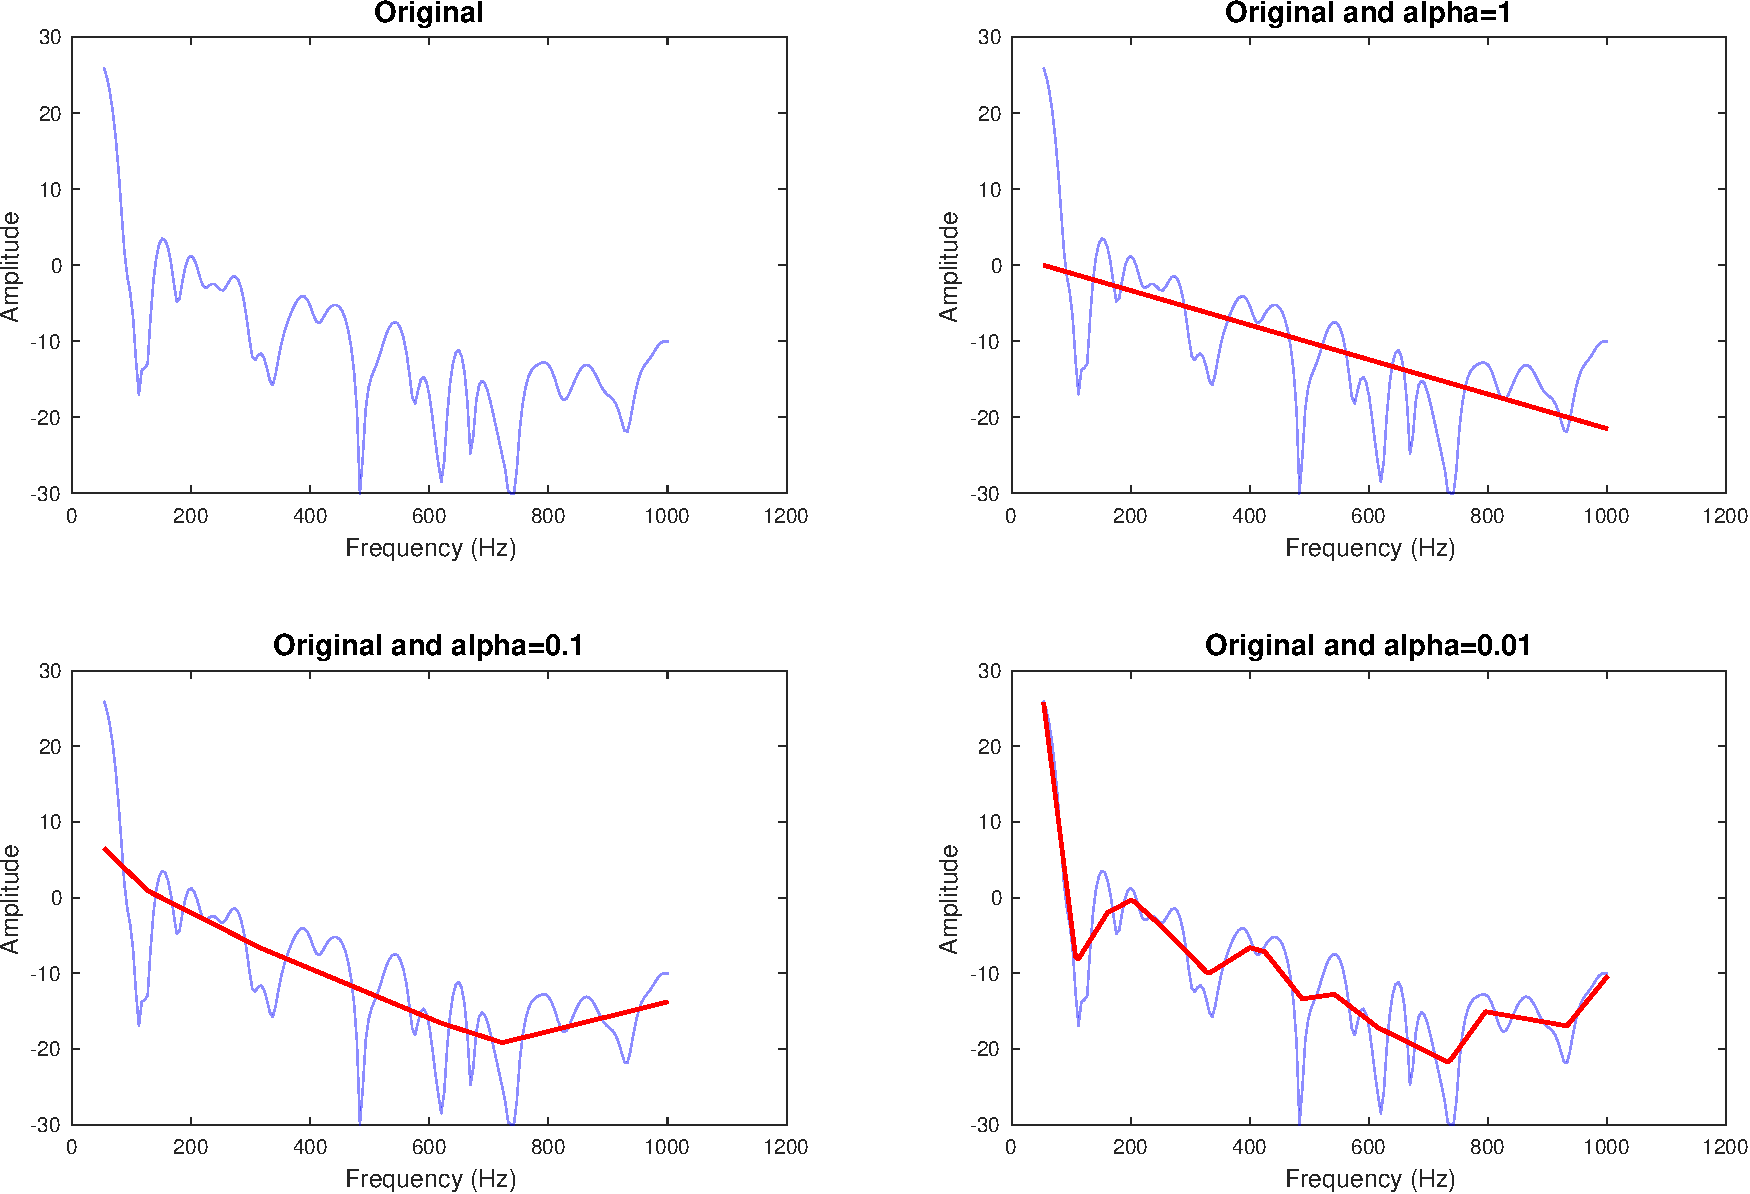
\includegraphics[width=0.95\textwidth]{img/ch5/example_l1_plots/segment_l1_trend.pdf}
        \caption{Overlay of a random time segment with its corresponding $\ell_1$ trend at various $\alpha$ values.}
        \label{fig:l1:segment-trend}
    \end{subfigure}
    
    \vspace{1cm}
    
    % Subfigure 2: Segment detrended plot
    \begin{subfigure}[t]{\textwidth}
        \centering
        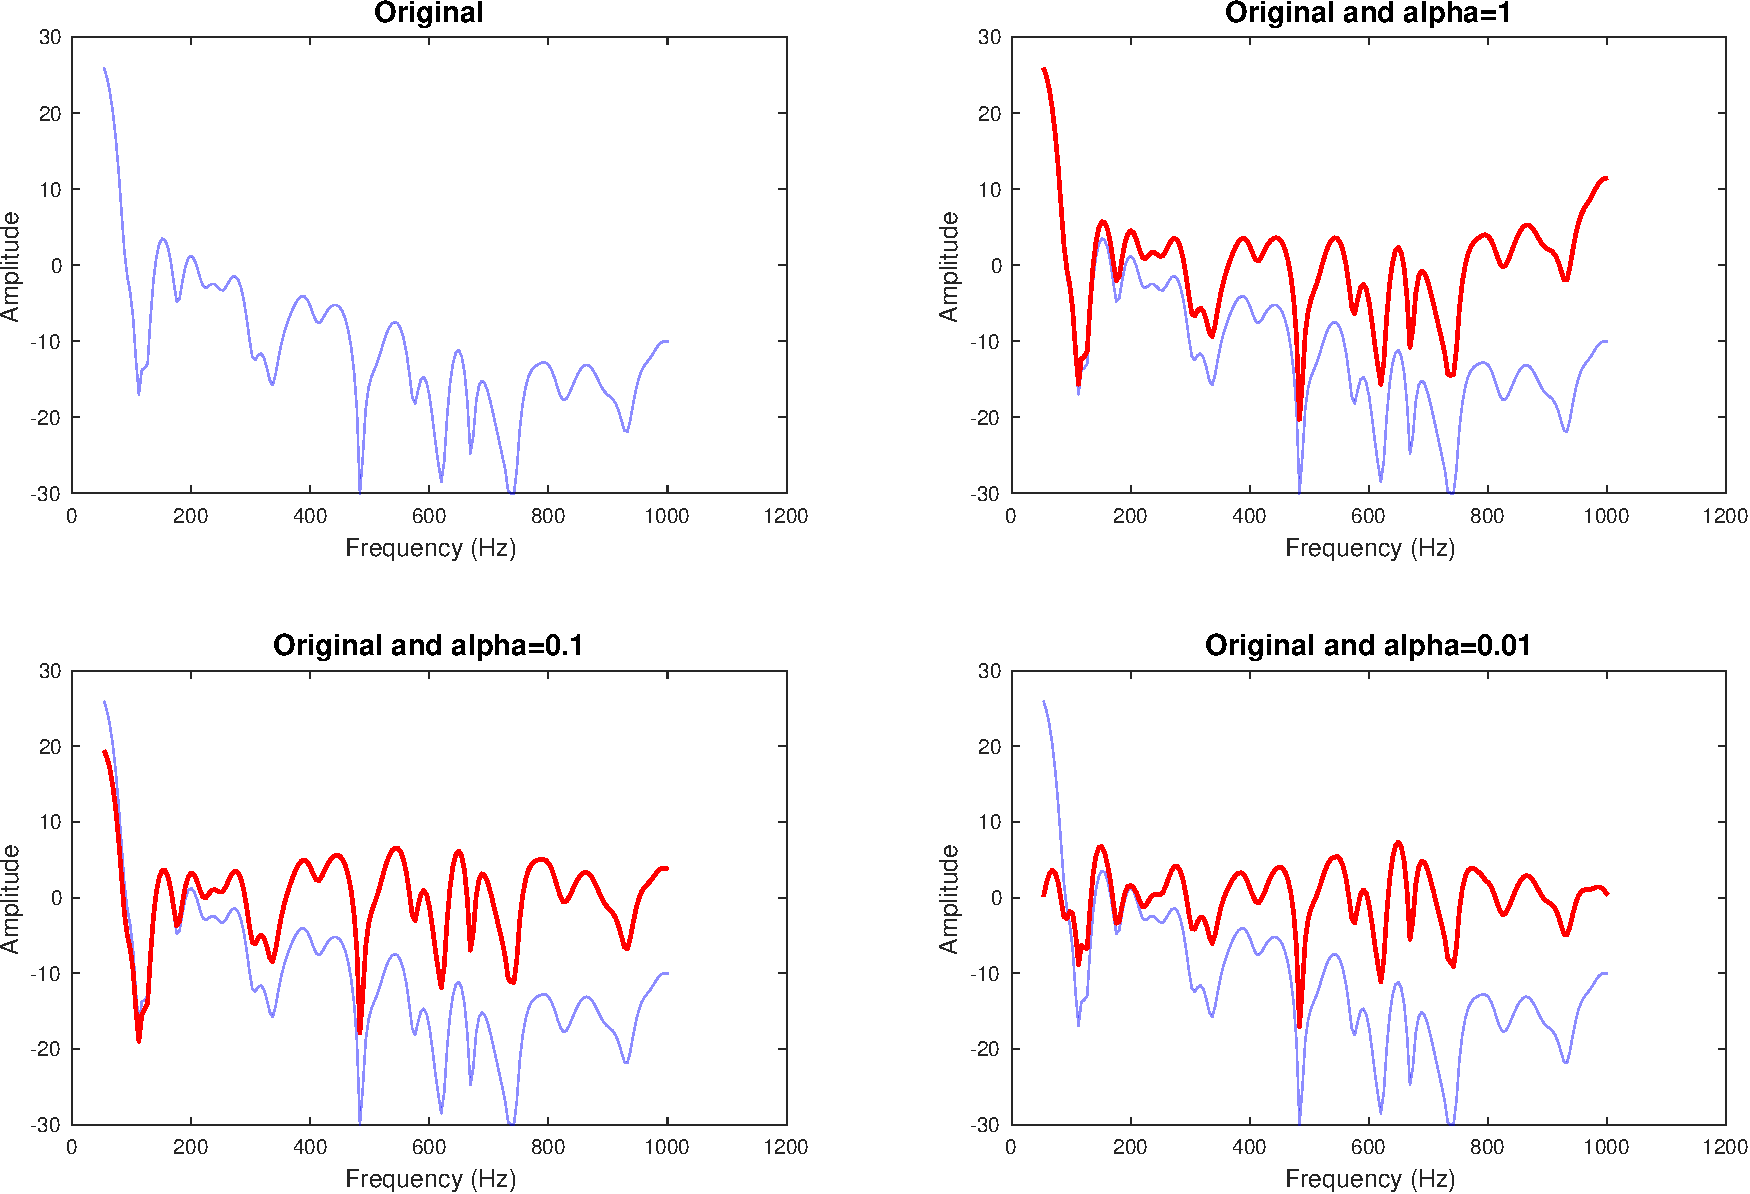
\includegraphics[width=0.95\textwidth]{img/ch5/example_l1_plots/segment_detrended.pdf}
        \caption{Random time segment before and after detrending at different $\alpha$ values, highlighting the removal of long-term trends in the signal.}
        \label{fig:l1:segment-detrended}
    \end{subfigure}
\end{figure}

\begin{figure}
    \ContinuedFloat
    % Subfigure 3: Spectrogram comparison
    \begin{subfigure}[t]{\textwidth}
        \centering
        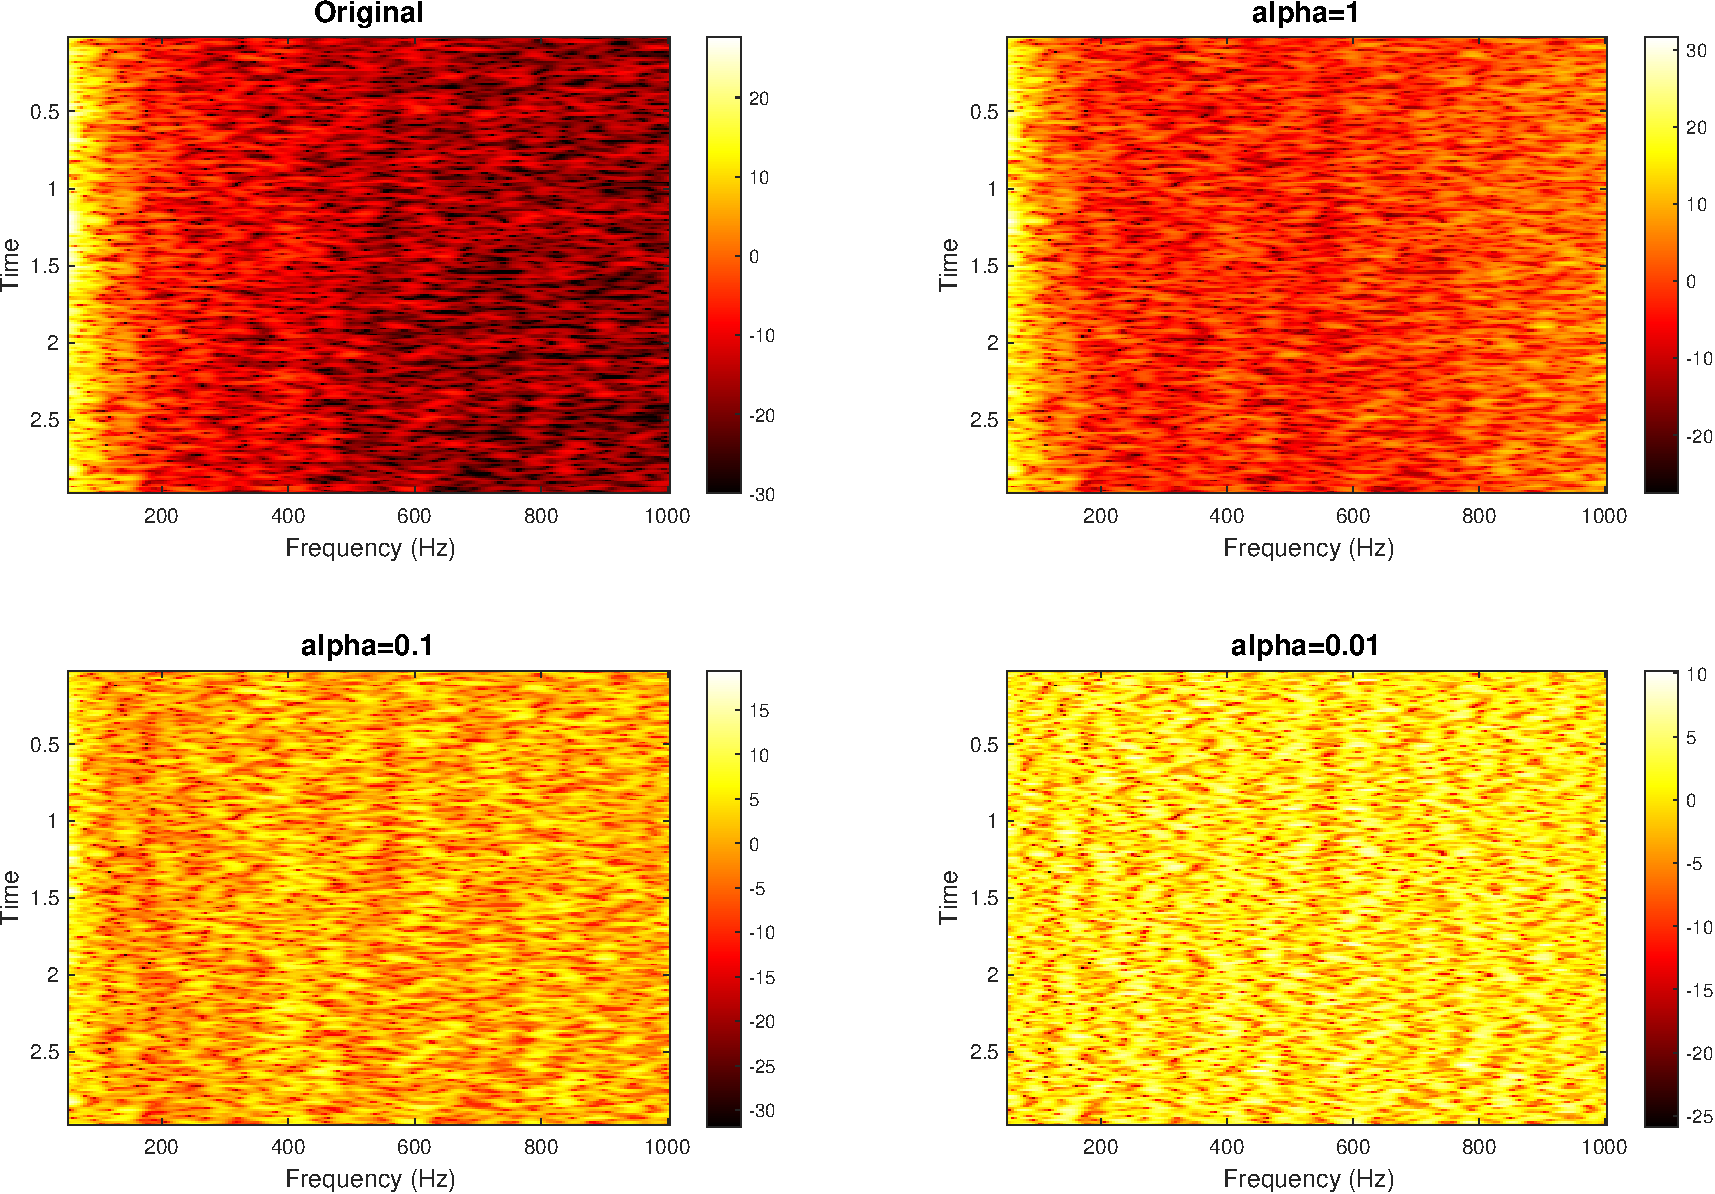
\includegraphics[width=0.92\textwidth]{img/ch5/example_l1_plots/spec_comparison.pdf}
        \caption{Comparison of original and detrended spectrograms produced using $\ell_1$ detrending at various $\alpha$ values.}
        \label{fig:l1:spectrogram-comparison}
    \end{subfigure}
    
    \vspace{1cm}
    
    % Subfigure 4: 3D surface plots
    \begin{subfigure}[t]{\textwidth}
        \centering
        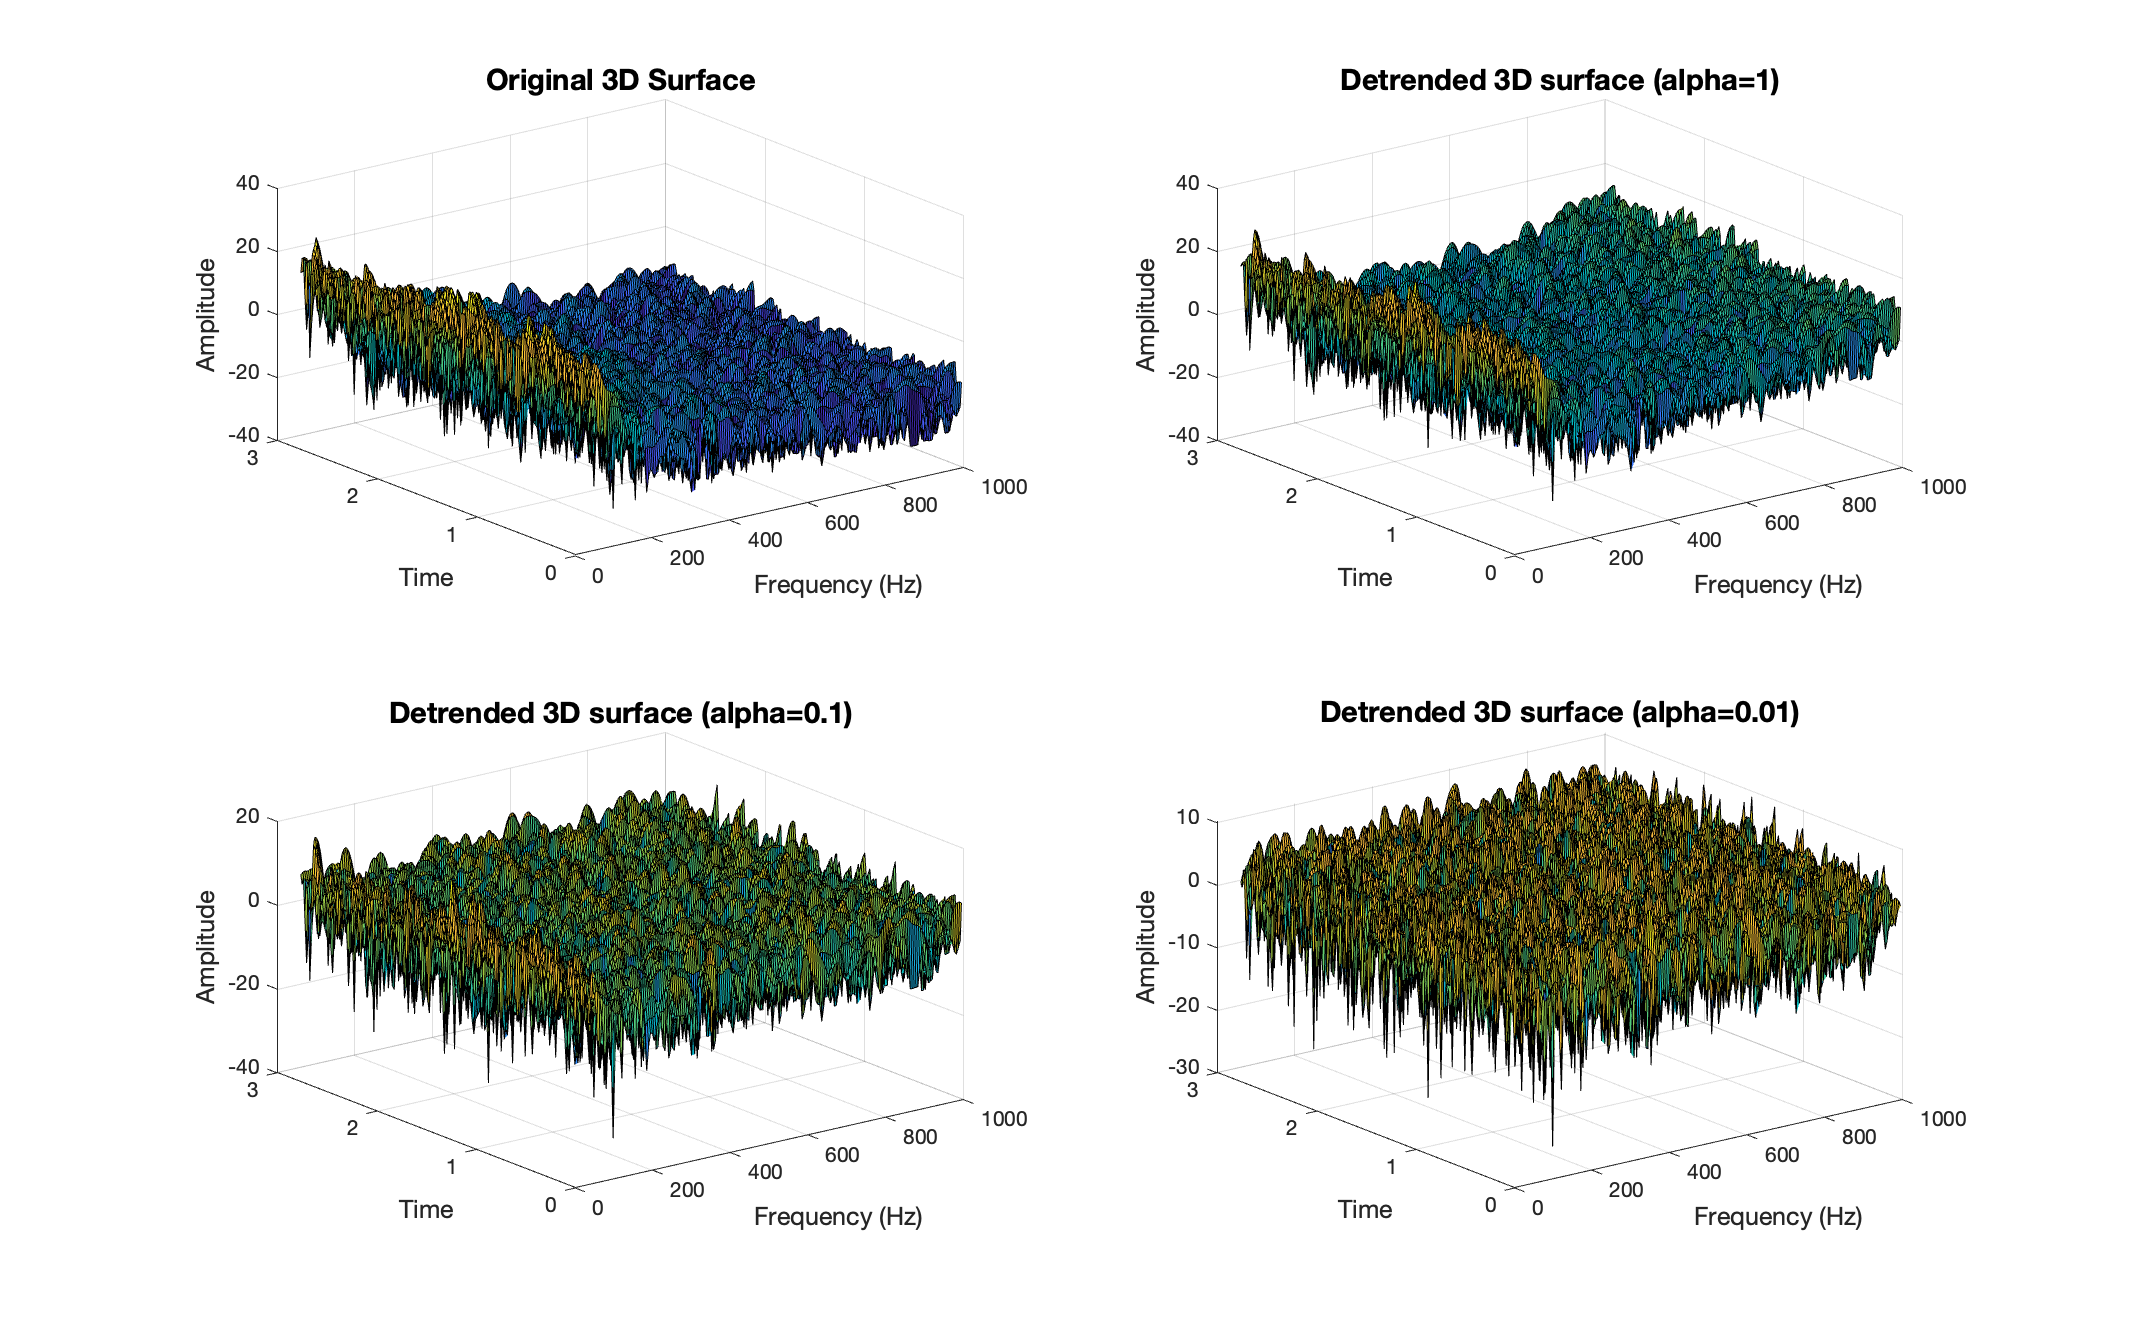
\includegraphics[trim={3cm 1.5cm 2.5cm 1cm},clip,width=0.92\textwidth]{img/ch5/example_l1_plots/3d_plot.pdf} %{left bottom right top}
        \caption{Three-dimensional surface plots of the original spectrogram and detrended spectrograms at different $\alpha$ values.}
        \label{fig:l1:3d}
    \end{subfigure}
    \caption{Visual analysis of $\ell_1$ detrending for various $\alpha$ values, illustrating its impact on spectrograms through comparative visualisations, time-segment overlays, and 3D surface plots.}
    \label{fig:l1:overview}
\end{figure}

To support this experimentation, our implementation of the $\ell_1$ detrending algorithm allows the user to specify up to 10 values of $\alpha$ in a single run. The function computes detrended spectrograms for each specified $\alpha$ value and generates a range of diagnostic plots that facilitate analysis. These visualisations were incredibly helpful in helping select appropriate values for $\alpha$ for subsequent experiments:
\begin{enumerate}
    \item Segment trend plot: This plot (Figure~\ref{fig:l1:segment-trend}) overlays a single random time segment with its corresponding $\ell_1$ trends for various $\alpha$ values. 
    \item Segment detrended plot: This diagnostic (Figure~\ref{fig:l1:segment-detrended}) shows the same time segment before and after detrending for various $\alpha$ values. It is the most helpful diagnostic plot to visualise the changes introduced by detrending, especially the removal of long-term trends such as those created by background noise .By examining the degree of smoothing introduced for different $\alpha$, we could evaluate how effectively the algorithm removed noise without discarding important signal features. Smaller $\alpha$ values were observed to retain more signal detail but were less effective at suppressing noise, while larger $\alpha$ values removed noise more aggressively but often smoothed out transient features.
    \item Spectrogram comparison: This diagnostic plot (Figure~\ref{fig:l1:spectrogram-comparison}) presents the original spectrogram alongside detrended spectrograms generated using different $\alpha$ values. It provides an overview of how detrending affects the overall amplitude structure, particularly in regions dominated by long-term trends or broadband noise. By visually assessing these plots, we could identify the boundaries where detrending was either too aggressive (overfitting) or too weak (underfitting).
    \item 3D surface plots: These 3D plots provide an alternative representation of how detrending impacts amplitude values across time and frequency (Figure \ref{fig:l1:3d}).
\end{enumerate}

Using these diagnostic plots, we determined that $\alpha$ values in the range $[10^{-3}, 1]$ provided a suitable balance between noise suppression and signal preservation. Hence, we chose three such $\alpha$ values for further experimentation: $10^{-2}$, $10^{-1},$ and $1$. These values were chosen in hopes of capturing a wide spectrum of detrending strengths, ranging from subtle noise suppression to more aggressive trend removal.

Hence, to evaluate the effect of $\ell_1$ detrending on UATR classification performance, the baseline 3-second DeepShip spectrograms (Section \ref{sec:inputs}) were processed using the three selected $\alpha$ values ($10^{-2}$, $10^{-1},$ and $1$). Each detrended spectrogram was saved to a separate directory as a \texttt{.mat} file and subsequently used as input to the CNN-LSTM baseline model. 

\subsection{Results}

The results, compared to the baseline model trained on non-detrended spectrograms, are presented in Table \ref{tab:detrend-results-3s}.

\begin{table}[htbp]
    \centering
    \caption{Classification results using $\ell_1$ detrending algorithm at various $\alpha$.}
    \label{tab:detrend-results-3s}
    \begin{tabular}{lcc}
        \toprule
        \textbf{Detrending parameter} & \textbf{Accuracy (\%)} & \textbf{Precision (\%)} \\ \midrule
        $\alpha = 10^{-2}$            & 48.22 & 59.09 \\
        $\alpha = 10^{-1}$            & 52.03 & 62.54 \\
        $\alpha = 1$                  & 55.63 & 63.97 \\
        \textbf{Baseline (no detrending)}  & \textbf{63.41} & \textbf{66.53} \\
        \bottomrule
    \end{tabular}
\end{table}


The results are quite underwhelming. Table \ref{tab:detrend-results-3s} shows that all three selected $\alpha$ values produced significantly lower classification accuracies and F1-scores compared to the baseline model trained on non-detrended spectrograms, with accuracy reductions of between 6.5 and 9.2\%. It is interesting to note that all three $\alpha$ values resulted in classification accuracies within a range less than 3\% of each other, with $\alpha = 10^{-2}$ achieving the \textit{same} classification accuracy as $\alpha = 1$. 

\subsection{Discussion}


This consistent drop in accuracy across all $\alpha$ values suggests that $\ell_1$ detrending, while effective at removing long-term trends, may also inadvertently be removing  or distorting features essential for classification, regardless of the chosen $\alpha$ value.

This performance drop may be attributed to several factors. Lower $\alpha$ values may be causing \textit{over-smoothing}; that is, the $\ell_1$ algorithm is aggressively suppressing broadband noise through the removal of the long-term trend, but also smoothing out transient narrowband features such as machinery noise -- key discriminators for different vessel types. On the other hand, higher $\alpha$ values may be preserving finer details while failing to adequately suppress broadband noise: a phenomenon called \textit{under-suppression}. Furthermore, it is possible that the short duration of the input segments (Section \ref{subsec:segmentation}) is preventing the $\ell_1$ algorithm from accurately capturing the broader trend of each recording. More fundamentally, it may simply be that through removing long-term trends, the detrended spectrograms are losing the distinct structure necessary for the baseline CNN-LSTM model to effectively discern between vessel types. 

The validation accuracy and loss curves (Figure~\ref{fig:detrend-acc-loss-curves-fold}) reinforce these findings, revealing erratic and unstable training dynamics. For $\alpha = 10^{-2}$, the validation loss spikes at folds 3 and 7 causing the validation accuracy to fluctuate significantly, suggesting poor generalisation and potential overfitting to noise in certain folds. The curve for $\alpha = 10^{-1}$, though less erratic than $\alpha = 10^{-2}$, still shows noticeable bumps in validation loss, particularly around folds 5 and 9. The model struggles to converge smoothly, which limits its effectiveness and applications. The training for $\alpha = 1$ displays the most stable curves, with fewer spikes and smoother transitions. However, the loss curve still shows a ``double minima'' at folds 5 and 10, suggesting inconsistencies in the optimisation process. These curves highlight the challenges in achieving stable performance with detrended spectrograms.

The above findings highlight the challenges of using $\ell_1$ detrending for UATR tasks and suggest several directions for future research. Perhaps the simplest next step would be to test $\alpha$ values outside the current range in hopes of identifying a configuration that better balances noise suppression and feature preservation. Secondly, it would be interesting to investigate the characteristics of those folds with an erratic validation loss, such as folds 3 and 7. An understanding of what makes these folds different, including any specific trends or noise patterns more prominent in these subsections of the dataset, could allow for a greater understanding of why the above experiment performed poorly. Thirdly, testing the detrending algorithm on longer segments of DeepShip recordings could see more accurate trend-capturing. Finally, a comparison of $\ell_1$ detrending with other detrending algorithms (such as wavelet detrending) would be insightful to determine whether achieving higher classification accuracy is achievable on this dataset.

\subsection{Conclusion}

While $\ell_1$ detrending holds promise for its ability to capture sharp transitions and suppress long-term trends, its application to \acrshort{uatr} tasks presents significant challenges. The observed drop in classification performance and erratic validation dynamics suggest that the current approach may not effectively balance noise suppression and feature retention. Further refinements or alternative preprocessing techniques will likely be necessary to achieve optimal results for \acrshort{uatr} classification.
